\documentclass[11pt,a4paper,twocolumn]{article}
\usepackage[utf8]{inputenc}
\usepackage{amsmath}
\usepackage{graphicx}
\usepackage{hyperref}
\usepackage{setspace}
\usepackage{enumerate}
\title{Assignment6}
\author{Aravind A Anil}
\date{\today}

\begin{document}

\maketitle
\begin{flushleft}
\textbf{Problem statement:}Find the probability distribution of number of success in two tosses of die,where success is defined as
\begin{enumerate}[i]
    \item number greater than 4
    \item six appear on at-least one die
\end{enumerate}
\section{number greater than 4}
Let X be the number of times the number greater than 4 occurs\\
When we throw 2 dies,there can be three cases
\begin{enumerate}
    \item no number greater than 4
    \item one number greater than 4
    \item both number greater than 4
\end{enumerate}
so values of \textbf{X} can be \textbf{0,1,2}\\
The sample space when 2 dies are thrown,
\begin{table}[h]
    \centering
    \begin{tabular}{|c|c|c|c|c|c|c|}
    \hline
         &1&2&3&4&5&6\\  
         \hline
         1&(1,1)&(1,2)&(1,3)&(1,4)&(1,5)&(1,6)\\
         \hline
         2&(2,1)&(2,2)&(2,3)&(2,4)&(2,5)&(2,6)\\
         \hline
         3&(3,1)&(3,2)&(3,3)&(3,4)&(3,5)&(3,6)\\
         \hline
         4&(4,1)&(4,2)&(4,3)&(4,4)&(4,5)&(4,6)\\
         \hline
         5&(5,1)&(5,2)&(5,3)&(5,4)&(5,5)&(5,6)\\
         \hline
         6&(6,1)&(6,2)&(6,3)&(6,4)&(6,5)&(6,6)\\
         \hline
         
    \end{tabular}
    \caption{\textbf{Sample space}}
\end{table}
\end{flushleft}
\begin{table}[ht]
\centering
    \begin{tabular}{|c|c|c|}
    \hline
        X &Number of outcomes&P(X)\\[5pt]
        \hline
    0&16&$\frac{16}{36}=\frac{4}{9}$\\[5pt]
    \hline
    1&16&$\frac{16}{36}=\frac{4}{9}$\\[5pt]
    \hline
    2&4&$\frac{4}{36}=\frac{1}{9}$\\[5pt]
    \hline
    \end{tabular}
    \caption{\textbf{Favourable outcomes}}
\end{table}
\begin{table}[ht]
    \centering
    \begin{tabular}{|c|c|c|c|}
    \hline
    X&0&1&2\\[5pt]
    \hline
    P(X)&$\frac{4}{9}$&$\frac{4}{9}$&$\frac{1}{9}$\\[5pt]
    \hline
    \end{tabular}
    \caption{\textbf{probability distribution}}
\end{table}
\begin{figure}[h!]
    \centering
    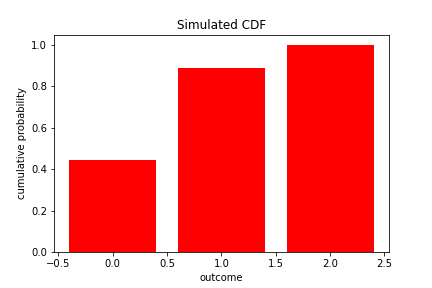
\includegraphics[width=10cm]{simulated CDF.png}
    \caption{simulated CDF}
\end{figure}
\begin{figure}[h!]
    \centering
    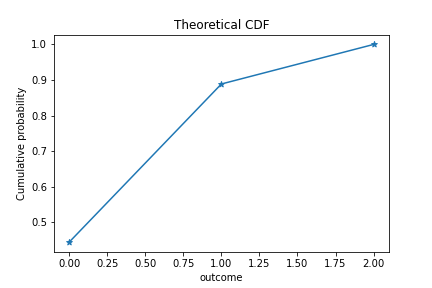
\includegraphics[width=8.25cm]{Theoretical CDF.png} 
    \caption{Theoretical CDF}
\end{figure}
\begin{figure}[h!]
    \centering
    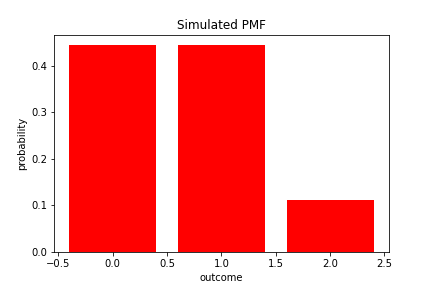
\includegraphics[width=8.25cm]{simulated PMF.png} 
    \caption{simulated PMF}
\end{figure}
\begin{figure}[h!]
    \centering
    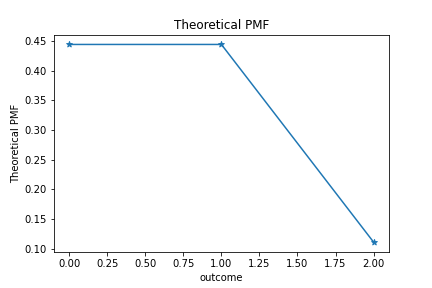
\includegraphics[width=8.25cm]{Theoretical PMF.png}
    \caption{theoretical PMF}
\end{figure}
\section{six appear on at-least one die}
since a pair of dies are thrown,\\
There can be two cases
\begin{enumerate}
    \item six does not appear at all
    \item six appear on atleast one die
\end{enumerate}
Hence,\\ X=0 six does not appears at all\\
X=1 appears on atleast die
\\ \textbf{Finding P(X=1)}\\
ie,probability that at-least one head appears
\begin{table}[h]
    \centering
    \begin{tabular}{|c|c|c|c|c|c|c|}
    \hline
         &1&2&3&4&5&6\\  
         \hline
         1&(1,1)&(1,2)&(1,3)&(1,4)&(1,5)&\textbf{(1,6)}\\
         \hline
         2&(2,1)&(2,2)&(2,3)&(2,4)&(2,5)&\textbf{(2,6)}\\
         \hline
         3&(3,1)&(3,2)&(3,3)&(3,4)&(3,5)&\textbf{(3,6)}\\
         \hline
         4&(4,1)&(4,2)&(4,3)&(4,4)&(4,5)&\textbf{(4,6)}\\
         \hline
         5&(5,1)&(5,2)&(5,3)&(5,4)&(5,5)&\textbf{(5,6)}\\
         \hline
         \textbf{6}&\textbf{(6,1)}&\textbf{(6,2)}&\textbf{(6,3)}&\textbf{(6,4)}&\textbf{(6,5)}&\textbf{(6,6)}\\
         \hline
         
    \end{tabular}
    \caption{\textbf{Sample space}}
\end{table}
\\[5pt]
P(X=1)=$\frac{11}{36}$\\[5pt]
\textbf{Finding P(X=0)}
\\i.e,probability that six does-not appear
\begin{align*}
    \text{P(X=0)}&=\text{probability that six does-not appear}\\
    &=1-\text{P(X=1)}\\
    &=1-\frac{11}{36}\\
    &=\frac{25}{36}
\end{align*}
Therefore,P(X=0)=$\frac{25}{36}$
so,our probability distribution is
\begin{table}[ht]
    \centering
    \begin{tabular}{|c|c|c|}
    \hline
         X&0&1  \\
         \hline
         P(X)&$\frac{25}{36}$&$\frac{11}{36}$\\[5pt]
         \hline
    \end{tabular}
    \caption{probability distribution}
    \label{tab:my_label}
\end{table}
\begin{figure}[h!]
    \centering
    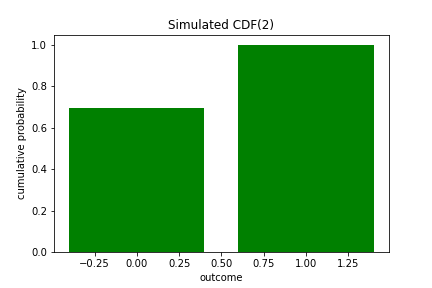
\includegraphics[width=9cm]{simulated CDF(2).png}
    \caption{simulated CDF}
\end{figure}
\begin{figure}[h!]
    \centering
    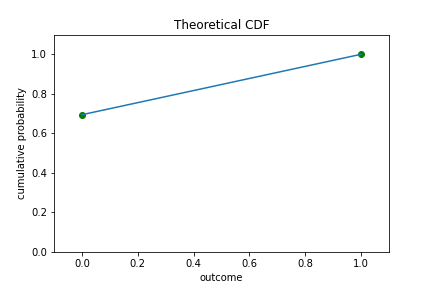
\includegraphics[width=9cm]{Theoretical CDF(2).png} 
    \caption{Theoretical CDF}
\end{figure}
\begin{figure}[h!]
    \centering
    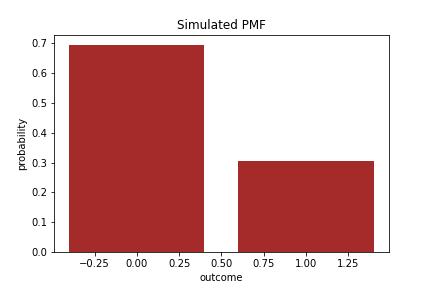
\includegraphics[width=9cm]{simulated PMF(2).png} 
    \caption{simulated PMF}
\end{figure}
\begin{figure}[h!]
    \centering
    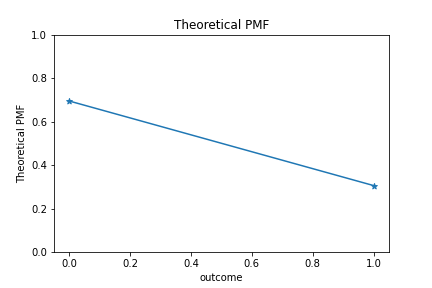
\includegraphics[width=9cm]{Theoretical PMF(2).png}
    \caption{theoretical PMF}
\end{figure}
\end{document}
